\documentclass[a4paper,12px]{article}
\usepackage{graphicx}
\usepackage[english]{babel}
\usepackage{fancyhdr}
\usepackage{lastpage}
\usepackage{xifthen}
\usepackage[linesnumberedhidden, titlenotnumbered]{algorithm2e}
\usepackage{lipsum}
\usepackage{hyperref}
\usepackage{array}
\usepackage{tabularx}
\usepackage{caption}
\usepackage{amsfonts}
\usepackage{amssymb}
\usepackage{amsmath}
\usepackage{placeins}
\usepackage{enumitem}

\usepackage{minted}
\usepackage{listings}
\usepackage{dsfont}
\usepackage{units}

\pagestyle{fancy}
\lhead{
\includegraphics[width=7cm]{logoUvA}}
\rhead{\footnotesize \textsc {Report\\ \opdracht}}
\lfoot
{%
    \footnotesize \studentA
    \ifthenelse{\isundefined{\studentB}}{}{\\ \studentB}
    \ifthenelse{\isundefined{\studentC}}{}{\\ \studentC}
    \ifthenelse{\isundefined{\studentD}}{}{\\ \studentD}
    \ifthenelse{\isundefined{\studentE}}{}{\\ \studentE}
}
\cfoot{}
\rfoot{\small \textsc {Page \thepage\ of \pageref{LastPage}}}
\renewcommand{\footrulewidth}{0.5pt}

\fancypagestyle{firststyle}
{%
    \fancyhf{}
    \renewcommand{\headrulewidth}{0pt}
    \chead{
\includegraphics[width=7cm]{logoUvA}}
    \rfoot{\small \textsc {Page \thepage\ of \pageref{LastPage}}}
}

\setlength{\topmargin}{-0.3in}
\setlength{\textheight}{630pt}
\setlength{\headsep}{40pt}
\setlength{\parindent}{0pt}

% =================================== DOC INFO ===================================

\newcommand{\opdracht}{Statistisch Redeneren}
\newcommand{\titel}{Lab 5}
\newcommand{\docent}{Rein van de Boomgaard}
\newcommand{\cursus}{Statistisch Redeneren}
\newcommand{\vakcode}{5062STRE6Y}
\newcommand{\datum}{\today}
\newcommand{\studentA}{Maico Timmerman}
\newcommand{\uvanetidA}{10542590}
\newcommand{\studentB}{Tim van Zalingen}
\newcommand{\uvanetidB}{10784012}
% \newcommand{\studentC}{Boudewijn Braams}
\newcommand{\uvanetidC}{10401040}
% \newcommand{\studentD}{Govert Verkes}
\newcommand{\uvanetidD}{10211748}
%\newcommand{\studentE}{Naam student 5}
\newcommand{\uvanetidE}{UvAnetID student 5}

% ===================================  ===================================

\begin{document}
\thispagestyle{firststyle}
\begin{center}
    \textsc{\Large \opdracht}\\[0.2cm]
    \rule{\linewidth}{0.5pt} \\[0.4cm]
    {\huge \bfseries \titel}
    \rule{\linewidth}{0.5pt} \\[0.2cm]
    {\large \datum  \\[0.4cm]}

    \begin{minipage}{0.4\textwidth}
        \begin{flushleft}

            \emph{Students:}\\
            {\studentA \\ {\small \uvanetidA \\[0.2cm]}}
            \ifthenelse{\isundefined{\studentB}}{}{\studentB \\ {\small \uvanetidB \\[0.2cm]}}
        \end{flushleft}
    \end{minipage}
    ~%
    \begin{minipage}{0.4\textwidth}
        \begin{flushright}
            \emph{Lecturer:} \\
            \docent \\[0.2cm]
            \emph{Course:} \\
            \cursus \\[0.2cm]
            % \emph{Student:}\\
            \ifthenelse{\isundefined{\studentC}}{}{\studentC \\ {\small \uvanetidC \\[0.2cm]}}
            \ifthenelse{\isundefined{\studentD}}{}{\studentD \\ {\small \uvanetidD \\[0.2cm]}}
            \ifthenelse{\isundefined{\studentE}}{}{\studentE \\ {\small \uvanetidE \\ [0.2cm]}}
        \end{flushright}
    \end{minipage}\\[1 cm]
\end{center}


% =================================== CONTENTS ===================================

\tableofcontents
\clearpage

% =================================== MAIN TEXT ===================================

\section{4.2: $k$-NNb classifier}
This is an example of the $k$-NNb classifier with $k=5$.
\begin{figure}[!h]
    \centering
    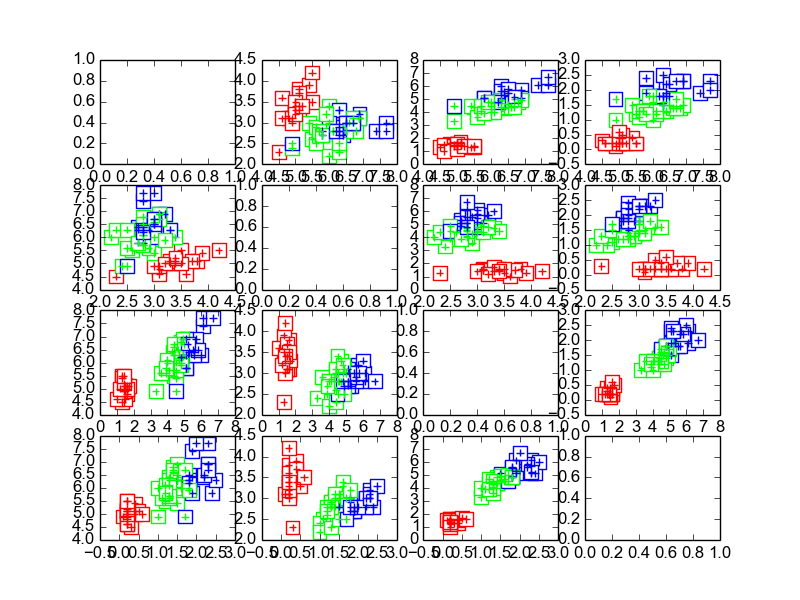
\includegraphics[width=1\textwidth]{knnb_example.png}
    \caption{$k$-NNb classifier with $k=5$.}
    \label{fig:knnb_example}
\end{figure}
\FloatBarrier
The accuracy of the classifier has been tested for each k of 1, 3, 5, 7 and 9.
 This has been tested by taking an average over 20 times of all rightly
 classified divided by the amount to be classified.
\begin{table}[h!]
\centering
\caption{The accuracy of each k tested 20 times.}
\label{my-label}
\begin{tabular}{|l|l|}
\hline
\textbf{k} & \textbf{accuracy}  \\ \hline
1          & 95.75\%            \\ \hline
3          & 96\%               \\ \hline
5          & 96.59\%            \\ \hline
7          & 96.83\%            \\ \hline
9          & 97.25\%            \\ \hline
\end{tabular}
\end{table}

\section{4.3: Minimum Error Classification I}
These are the class boundaries:
\begin{equation}
    \begin{aligned}
        P(C=1|X) &= \dfrac{P_{XC}(x,C=1)}{P_{XC}(x,C=1)+ P_{XC}(x,C=2)}\\
        P(C=2|X) &= \dfrac{P_{XC}(x,C=2)}{P_{XC}(x,C=1)+ P_{XC}(x,C=2)}
    \end{aligned}
\end{equation}
\begin{figure}[h!]
    \centering
    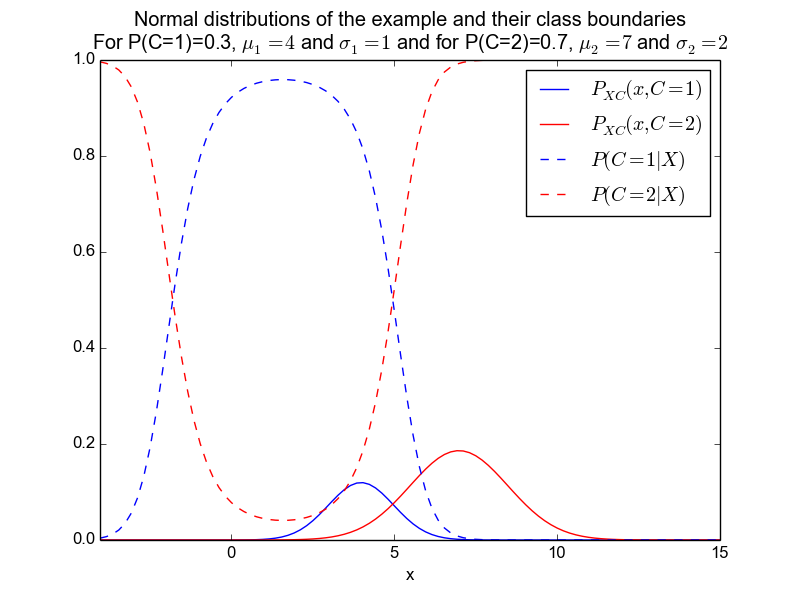
\includegraphics[width=1\textwidth]{min_err_class.png}
    \caption{Minimum error classification.}
    \label{fig:knnb_example}
\end{figure}
\FloatBarrier

\section{4.4: Minimum Error Classification II}
The MAP classifier works by calculating the mean vector and covariance matrix for
 each set of iris data.

For each of these sets with their mean vector and covariance matrix, the
multivariate normal distribution is calculated, using the following formula.

\begin{equation}
    \begin{aligned}
        f_{\mathbf x}(x_1,\ldots,x_k) =
        \frac{1}{\sqrt{(2\pi)^{k}\det{\boldsymbol\Sigma}}}
        \exp\left(-\frac{1}{2}(x-\mu)^T\Sigma^{-1}(x-\mu)
    \right)
    \end{aligned}
\end{equation}

For each entry of the test data, the probability of all iris types is calculated
from this distribution. The iris with the highest probability is set as the
corresponding iris.

The MAP classifier running over the iris dataset achieves an accuracy of
0.972244 for 60060 tests (58393 correct).

% =================================== REFERENCES ===================================

%\clearpage
% \bibliographystyle{apalike}
% \bibliography{report}

\end{document}
